\chapter{System Design}



\section{System Overview}
As a means to both explaining the system and as a practical development model,
the system can be thought of as being made up of layers.
Each layer being an abstraction of workings in the layers beneath it,
with the partitions at the top and the hardware at the bottom.
This model is defined by the ARINC 653 standard
\todo[inline,color=green]{Insert ref to analysis of ARINC.}
and expanded upon here with drivers being build on top of the HAL library,
instead of directly on top of the hardware,
creating an extra layer of abstraction.

\begin{itemize}
	\item \textbf{Partitions}
		are running the applications which defines how the system interacts
		with the system around it.
		Doing so in complete isolation from one another.
	\item \textbf{APEX}
		defines the methods by which the partitions talk to the world and
		interacts with other partitions or systems, running
		on the same chip or otherwise connected.
	\item \textbf{OS}
		provides the infrastructure of partitions to operate and
		including scheduling.
	\item \textbf{Drivers}
		serves the OS with methods to create an enviroment in which partitions
		can be run and scheduled without affection one another.
	\item \textbf{HAL}
		An abstraction layer provided by the chip manufacturer,
		to make setting up the hardware easier on developers.
	\item \textbf{Hardware}
		The physical platform on which everything is executed.
\end{itemize}

An XML file is provided by the system developer at compile time.
It defines how the top layers interact and set the requirements of the drivers
and the underlying hardware.

Every layer contains a list of components, which provides the functionalities
of that layer.
Beneath graphical overview of the different layers with their core components
is provided.

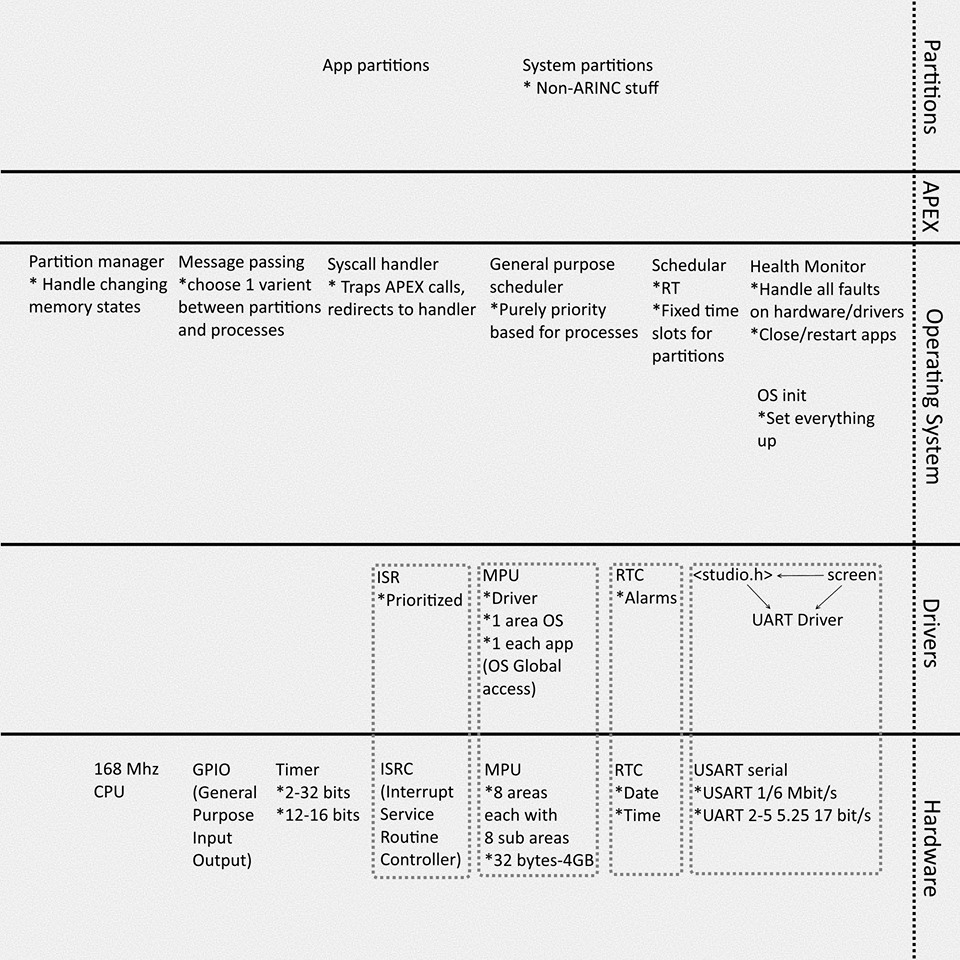
\includegraphics[width=13cm]{first_draft_sys_design_diag.jpeg}

In the rest of the chapter the different layers are described with their core
components together with an overall view in the specifications for the hardware
and the XML.


\subsection{Hardware}

\subsection{Drivers}
\begin{description}[align=left]
	\item [\textbf{UART driver}] The UART is used by the system to communicate with the outside
	world. This can either receive or transmit data to another UART device.
	\item [\textbf{Watchdog timer driver}] The watchdog timer is necessary to ensure recovery
	in case of a hardware fault or program error. If this happens, the program would be restarted
	from a safe state.

\end{description}

\subsection{OS}
\begin{description}[align=left]
	\item [\textbf{scheduler}] more text
	\item [\textbf{scheduler}] a whole lot of words
\end{description}
\subsubsection{Interpartition communication}

\section{XML}


\section{Memory Management}
ARINC 653 advertizes time and space seperation covered in (ref to sec in analysis).
To accommodate for the feature of seperating partitions in space
this operating system relies on the memory management unit (MPU)
to manage permissions accross sections of memory
ensuring that partitions stay within a dedicated memory space.

\subsection{something about ARINC on memory management}

\subsection{the MPU on a STM32F415}

\subsection{memory strategy}
